\documentclass[12pt]{article}
\usepackage[svgnames,x11names,table]{xcolor}
\usepackage{hyperref}
\usepackage{graphicx}
\usepackage{parskip}
\usepackage{float}
\usepackage{amsmath}
\usepackage{amssymb}
\usepackage{enumitem}
\usepackage[thicklines]{cancel}

\hypersetup{
    colorlinks,
    citecolor=blue,
    filecolor=black,
    linkcolor=black,
    urlcolor=RoyalBlue4,
}

\title{PEU 218 Assignment 5}
\author{Mohamed Hussien El-Deeb (201900052)}
\date{\today}

\DeclareMathOperator{\sech}{sech}
\DeclareMathOperator{\csch}{csch}

\begin{document}

\maketitle
\tableofcontents
\hypersetup{linkcolor=RoyalBlue4}

\newpage
\section{Question 1}

\subsection{Problem}

Use the Divergence theorem to evaluate \(\iint_S \vec{F} \cdot d \vec{S}\) where \(\vec{F}=\sin (\pi x) \hat{\imath}+z y^3 \hat{\jmath}+\left(z^2+4 x\right) \hat{k}\) and \(S\) is the surface of the box with \(-1 \leq x \leq 2,0 \leq y \leq 1\) and \(1 \leq z \leq 4\). Note that all six sides of the box are included in \(S\).

\subsection{Solution}

\newpage
\section{Question 2}

\subsection{Problem}

Use Stokes' theorem to evaluate \(\int_C \vec{F} \cdot d \vec{r}\) where \(\vec{F}=\left(3 y x^2+z^3\right) \hat{\imath}+y^2 \hat{\jmath}+4 y x^2 \hat{k}\) and \(C\) is the triangle with vertices \((0,0,3),(0,2,0)\) and \((4,0,0)\). \(C\) has a counter clockwise rotation if you are above the triangle and looking towards the \(x y\)-plane. See the figure below for a sketch of the curve

\begin{figure}[H]
    \centering
    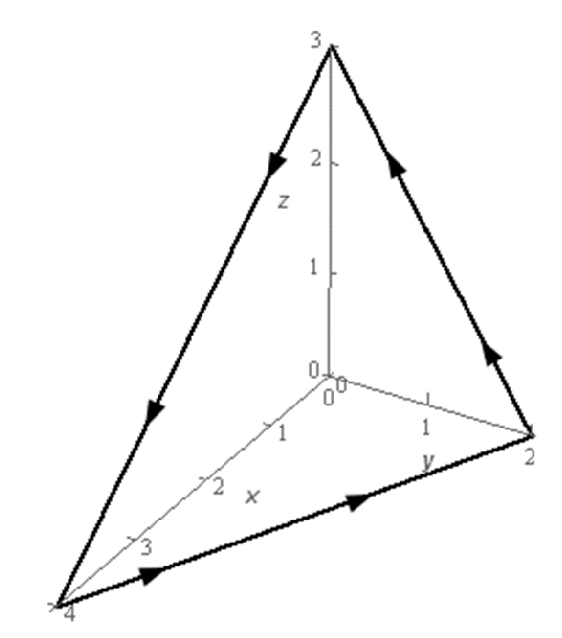
\includegraphics[width=0.5\textwidth]{Q2.png}
\end{figure}

\subsection{Solution}



\newpage
\section{Question 3}

\subsection{Problem}

Evaluate the line integral

\[
    I=\oint_C\left[y\left(4 x^2+y^2\right) d x+x\left(2 x^2+3 y^2\right) d y\right]
\]

around the ellipse \(\frac{x^2}{a^2}+\frac{y^2}{b^2}=1\)

\subsection{Solution}



\newpage
\bibliographystyle{plain}
\bibliography{references}
\nocite{El-Deeb_PEU-218_Assignments}

\end{document}